\section{チャネルを使ったコンポーネントの接続}

コンポーネントは、プロデューサコンポーネントからコンシューマコンポーネントに値を供給するために、継続的な一連の値を渡すために接続する必要があるかもしれません。 \texttt{core.async} チャネルは、このような目的に最適です。コンポーネントが値の入出力にチャネルを必要とする場合、そのコンポーネントは外部のチャネルを受け入れるか、内部でチャネルを作成して利用できるようにします。

例えば、ソーシャルメディアからのメッセージを受信するコンポーネントがあるとします。一つの選択肢は、コンポーネントがその構成の一部として着信チャネルを受け入れることでしょう。

\begin{lstlisting}[numbers=none]
(defn make-feed-processor
  "指定された入力チャネルに新しいフィードプロセッサを作成します。"
  [input-channel] ,,,)  
\end{lstlisting}

あるいは、feed-processorが自らチャネルを構築し、ユーザーがそれを要求できるようにすることもできます。

\begin{lstlisting}[numbers=none]
(defn make-feed-processor
  "新しいFeed Processorを作成する"
  []
  (let [ch (async/chan 100)] ,,,))

(defn input-chan
  "feed processorの入力チャネルを返します。"
  [feed-processor] ,,,)
\end{lstlisting}


ほとんどの場合、外部チャネルを受け入れることで、第7章「アプリケーションの構成」で説明するように、後でシステムを組み立てるための最も多くのオプションが生まれます。ここで決定すべき重要なことのひとつに、入力チャネルのバッファリングポリシーがあります。もしコンポーネントが内部で入力チャネルを作成するのであれば、この決定を行わなければなりません。もし設定可能である必要があるのなら、コンポーネントはバッファ設定オプションを公開する必要があります。チャネルを外部で作成する場合は、システムのアセンブリコードがシステムの残りの部分と一緒に自由に設定することができます。

どちらの場合でも、チャネルを持つコンポーネントができたら、それらをさまざまな方法で接続する必要があります。\texttt{core.async}は多くの種類のチャネルコネクタを提供します。ここでは、それらを直接接続、ファンイン、ファンアウトの観点から分類してみます。

\subsection{ダイレクトコネクション(1対1)}

内部で構築されたチャネルを提供する2つのコンポーネントを組み合わせる場合、直接接続が必要になることがあります。2つのコンポーネントを一緒に使うには、この例のようにチャンネルをパイプで接続します。


\begin{lstlisting}[numbers=none]
(let [component1 (make-comp-1)
      output-chan (get-output component1)
      component2 (make-comp-2)
      input-chan (get-input component2)]
  (pipe output-chan input-chan))
\end{lstlisting}

ここでは、 \texttt{component1} が出力チャネル、 \texttt{component2} が入力チャネルで、両者をパイプでつないでいます。デフォルトでは、最初のチャネルが閉じられると、2番目のチャネルも閉じられ、効果的にこれら2つのチャネルを1つのチャネルにまとめ、プロデューサー用に使用されます。この自動閉鎖の動作は、最後にオプションのブール値フラグを指定することで無効にすることができます。

しかし、消費者側から見ると、消費者が 2 番目のチャネルを閉じた場合、1 番目のチャネルは入力の消費を停止しますが、閉じることはありません。長く接続されているコンポーネントでは、この違いは重要ではないかもしれません。しかし、1つのチャネルとパイプで接続された2つのチャネルの違いの1つは、この違いです。コンポーネントが外部で構築されたチャネルを使用している場合、中間パイプを必要とせずに、あるコンポーネントと別のコンポーネントを直接接続するようにシステムを組み立てることができます。

パイプラインで見たように、 \texttt{core.async} は \texttt{pipeline} 関数も提供しており、それを使って2つのパイプを並列変換ステージで繋ぐことができます。

\subsection{ファンアウト(1対多)}

\texttt{core.async}ライブラリを使うと、チャネル上のメッセージを多くのコンシューマに簡単に公開することができます。ファンアウトする最も一般的な理由は、独立したコンシューマが異なる目的でメッセージを処理できるようにすることです(先の例では、ロギングとセンチメント分析のように)。\texttt{core.async} ライブラリはこれを行うためのいくつかの方法を提供します: \texttt{split}, \texttt{mult}, \texttt{pub/sub}.


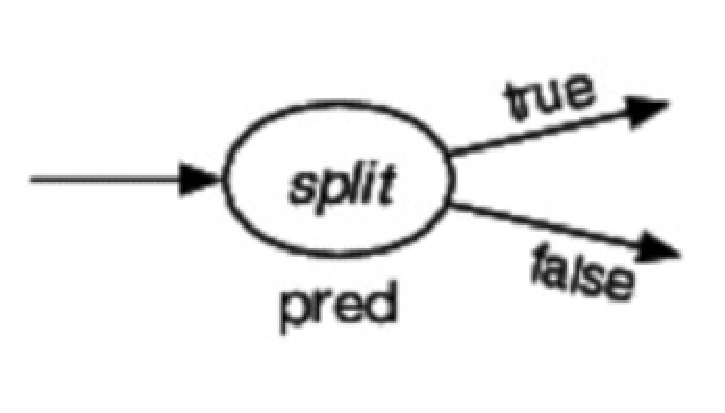
\includegraphics[width=8cm]{fig_06_003.eps}


\texttt{core.async}の \texttt{split} 関数は、1つのチャネルを受け取り、述語の真偽に基づいてトラフィックを2つの出力チャネルに分割します。これは図に示すとおりです。

例えば、\texttt{split} はストリームから無効なメッセージを分割し、別のプロセスに送って処理するのに適した方法です。


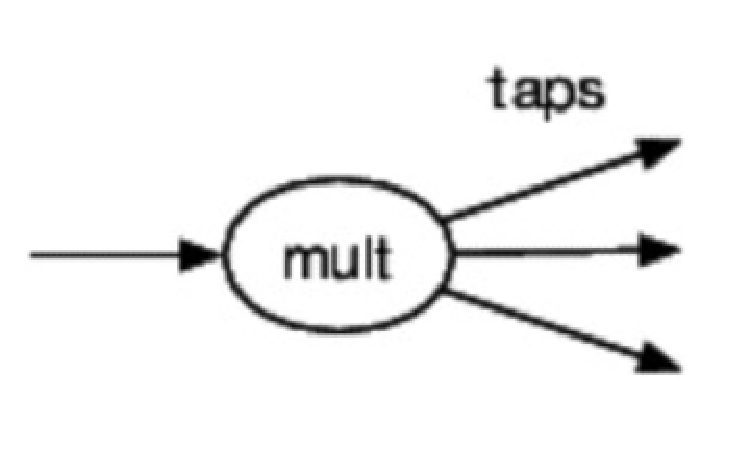
\includegraphics[width=8cm]{fig_06_004.eps}

\texttt{core.async}の \texttt{mult} 抽象化は、入力チャネルを受け取り、それを複数の出力チャネルに乗算します。

入力チャネルから項目が読み込まれると、次の値に移る前にすべての出力チャネルに供給されます。タップは \texttt{tap} 関数で \texttt{mult} に追加され(\texttt{untap} で削除され)ます。タップが閉じていることが判明した場合、そのタップは mult から削除されます。

すべてのチャネルが各値を受信する必要があるため、1つの遅いタップが \texttt{mult} を停止させる可能性があります。そこで、別のバッファリング戦略を使用することが有効です。例えば、パイプラインの特定の部分の出力ストリームをタップしてログにシャントし、何が起こっているかを覗き見ることができるようにしたいとします。

この関数は、入力と出力のチャネルを接続します( \texttt{pipe} で行ったことと同様です)が、返されるログのタップもインストールします。


\begin{lstlisting}[numbers=none]
(defn connect-and-tap
  "入力と出力を接続し、その間を流れるチャネルロギングデータを返します。"
  [input output]
  (let [m (mult input)
       log (chan (dropping-buffer 100))]
    (tap m output)
    (tap m log)
    log))
\end{lstlisting}

ここで重要なことは、ロギングチャネルが \texttt{droping-buffer} で作成されていることです。もしロギングチャンネルが追いつかないようなら、入ってくるメッセージはドロップされます。悲しいことに、私たちはそれらをログで見ることはできませんが、幸せなことに、私たちのシステムは稼働し続け、動作し続けます。これは、未束縛のバッファがないために、ジャンクでいっぱいのログバッファで夜中にプロセスが死ぬのではなく、早期にこれらのシナリオについて考えることを余儀なくされる良い例です。

\texttt{mult} 抽象は、すべてのメッセージをすべての \texttt{tap} に提供します。しかし、 \texttt{tap} が自分にとって適切なメッセージだけを受け取るようなメッセージバスが必要な場合はどうでしょうか? \texttt{core.async} はまさにこのような場合のために \texttt{pub/sub} 抽象化も提供しています。 \texttt{pub} 関数は、指定されたトピック関数を持つ公開チャネルを作成するために使用されます。\texttt{split} と同様に、トピック関数は各メッセージに適用され、値を返す必要がありますが、その値は何でもかまいません。 \texttt{sub} 関数は、トピック(トピック関数から返される値)上の \texttt{pub} に出力チャネルをサブスクライブするために使用されます。

例えば、ここでは \texttt{:topic} キー (関数として) を使用して、各マップ (またはレコード) メッセージのトピックを検索する \texttt{pub} があります。2 つの出力チャネル ( \texttt{news-ch} と \texttt{weather-ch} ) は、それぞれトピック \texttt{:news} と \texttt{:weather} でサブスクライブされています。

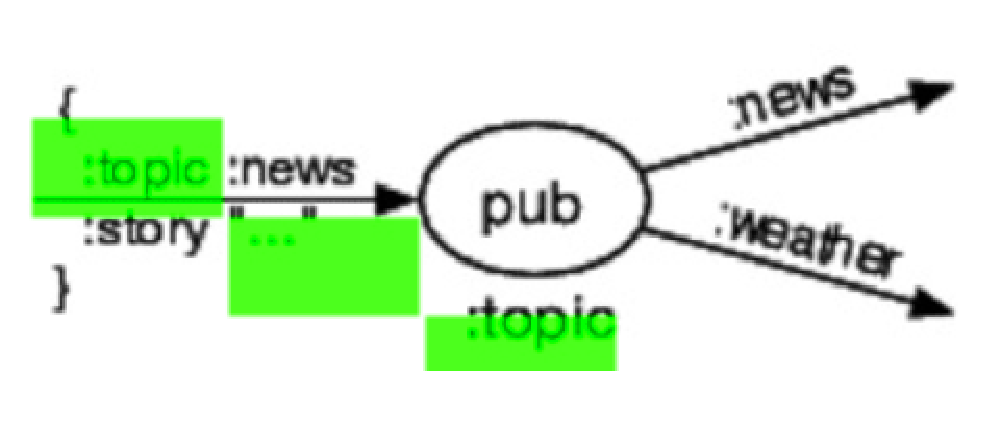
\includegraphics[width=8cm]{fig_06_005.eps}

\begin{lstlisting}[numbers=none]
(defn assemble-chans []
  (let [in (chan 10)
        p (pub in :topic)
        news-ch (chan 10)
        weather-ch (chan 10)]
    (sub p :news news-ch)
    (sub p :weather weather-ch)
    [in news-ch weather-ch]))
\end{lstlisting}

メッセージの \texttt{:topic} に \texttt{:news} が含まれる場合、\texttt{news-ch} に送信されます。トピックに \texttt{:weather} を含むメッセージは、\texttt{weather-ch} に送信されます。

チャネルは動的にサブスクライブとアンサブスクライブを行うことができ、これは有能なインメモリメッセージバスとなります。

さて、一つの入力チャネルを複数の出力チャンネルに分岐させる方法を見てきましたが、今度は多くの入力から一つの出力に分岐させる方法を考えてみましょう。

\subsection{ファンイン(Many-to-One)}

\texttt{merge} と \texttt{mix} は、多くの受信メッセージを単一の線形出力ストリームに結合するための 2 つのレベルの機能を提供します。

まず、より単純な \texttt{merge} を考えてみましょう。これは、任意の入力チャンネルに到着したすべてのメッセージを、単一の出力メッセージのストリームに単純に結合するものです。

\begin{lstlisting}[numbers=none]
(defn combine-channels
  [twitter-channel facebook-channel]
  (merge [twitter-channel facebook-channel] 100))
\end{lstlisting}

マージは下図のように表現されます。

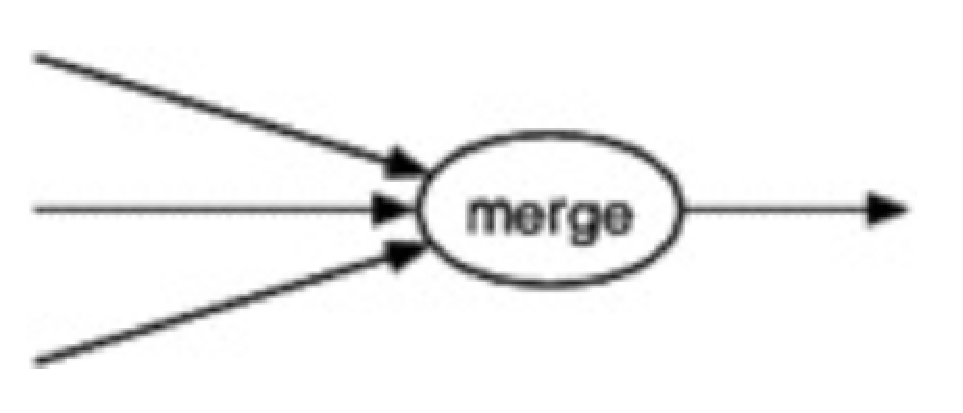
\includegraphics[width=8cm]{fig_06_006.eps}

チャネルの収集の後,\texttt{chan} と同様に出力チャネルにバッファまたは固定サイズバッファのチャネル設定を与えることができることに注意してください.マージされたチャネルは,作成後に変更することはできません.

多数のチャンネルを結合する場合、\texttt{mix} はオーディオミキサーのように動作し、下図のように各入力から出力チャネルに送られるメッセージのミックスを制御することができるようになります。

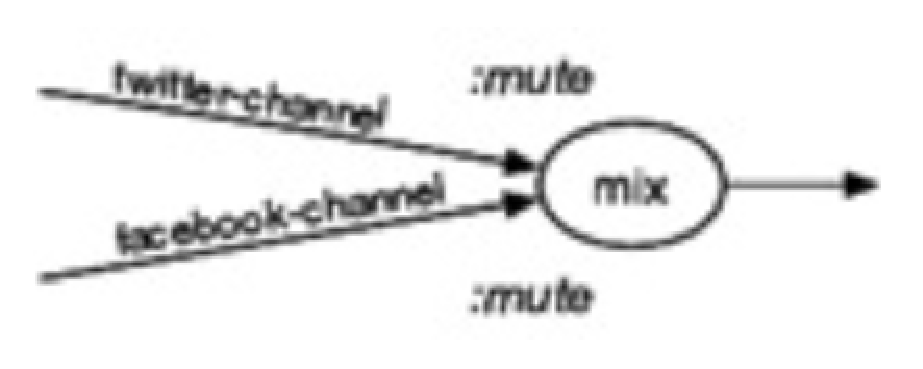
\includegraphics[width=8cm]{fig_06_007.eps}

入力チャンネルは \texttt{admix} で動的に追加し、 \texttt{unmix} で削除することができます。各入力チャネルは3つのトグル可能なモードを持っています。
\begin{itemize}
\item \texttt{:pause}-入力チャネルを消費せず、出力チャネルに含めない。

\item \texttt{:mute}-入力チャネルを消費し、出力チャネルには含めない。

\item \texttt{:solo}-True の場合、出力チャネルミックスにはソロ化されたチャネルのみが含まれます(この場合、pause と mute の設定は無視されます)。
\end{itemize}

これらのフラグはすべて、\texttt{toggle} 関数によって入力チャネルごとに設定することができます。

\begin{lstlisting}[numbers=none]
(defn mix-channels
      [twitter-channel facebook-channel out]
  (let [m (mix out)]
    (admix m twitter-channel)
    (admix m facebook-channel)
    (toggle m {twitter-channel {:mute true}
               facebook-channel {:mute true}})
    m))
\end{lstlisting}

このミックスは、両方のチャネルがミュートされた状態で作成されています。つまり、それらの入力は含まれずに読み込まれ、落とされることになります。

ソロモードのトグルを設定することで、そのうちの1つのチャネルをソロにすることができます。

\begin{lstlisting}[numbers=none]
(toggle m {twitter-channel {:solo true}})
\end{lstlisting}

入力チャネルのトグルの設定に加えて、出力チャネルのソロモードの状態を \texttt{solo-mode} で設定することが可能です。これは \texttt{:mute} または \texttt{:pause} に設定することができ、ソロになった入力チャネルをミュートまたは一時停止します。

ここまでで、 \texttt{core.async} の組み込みプリミティブを使用したチャネル接続の方法をすべて網羅しました。いくつかのケースでは、入出力チャネルの両端にアクセスすることで、接続方法を選択したり(例えば、ロギングタップを挿入する)、中間プロセスなしで同じ接続を使用したりすることができるようになります。両方の理由から、コンポーネント内でチャネルを作成するのではなく、通常、構成の一部としてチャネルを受け入れることをお勧めします。

さて、コンポーネントAPIの外面を設計する方法について見てきましたが、コンポーネントを実装する方法について、より細かい点を考えてみましょう。



